\documentclass[12pt]{report}
\usepackage[T1]{fontenc}
\usepackage[utf8]{inputenc}
\usepackage[polish]{babel}
\usepackage{geometry}
\geometry{a4paper, margin=1in}
\usepackage{tocbibind}
\usepackage{hyperref}
\usepackage{graphicx}
\usepackage{float}

\title{Narzędzie wspierające tworzenie testów dla aplikacji webowych}
\author{
    Łukasz Kowalewski \\ % Autor pracy
    \vspace{0.5cm} % Odstęp między autorem a promotorem
    Promotor: dr inż. Marcin Adamski % Promotor
}
\date{}

\begin{document}

\maketitle

\tableofcontents
\newpage

\chapter{Wstęp}
W niniejszym wstępie zostanie uzasadniona istotność tematu pracy inżynierskiej. Tytuł pracy -- \emph{Narzędzie wspierające tworzenie testów dla aplikacji webowych} -- wskazuje główną funkcję tworzonego w jej ramach programu. Jego rolą jest dostarczenie użytkownikom narzędzia pozwalającego przygotowywać oprogramowanie i testy w krótszym czasie przy zachowaniu wysokiej jakości. W kolejnych rozdziałach omówione zostaną motywacje, problematyka zagadnienia oraz możliwe rozwiązania. Aby zrozumieć powody podjęcia takiego tematu, należy wykazać potrzebę tworzenia oprogramowania wspierającego proces testowania.

Testy stanowią kluczowy element zaawansowanych i dojrzałych systemów informatycznych oraz aplikacji. W dużych korporacjach istnieją specjalne działy zajmujące się wyłącznie tworzeniem i utrzymywaniem testów, a sam rynek pracy sygnalizuje wysoki popyt na programistów wyspecjalizowanych w tym obszarze. W takich organizacjach powstają zaawansowane narzędzia do automatyzacji testów, co jest zrozumiałe w kontekście ogromnych strat finansowych, jakie mogą wynikać z błędów w krytycznym oprogramowaniu.

Odmiennie sytuacja bywa postrzegana w małych i średnich projektach, gdzie często brakuje dostatecznej motywacji (np. w postaci wysokich strat finansowych), by inwestować czas w rozbudowaną automatyzację testów. Celem tworzonej aplikacji jest ułatwienie generowania prostych testów w krótkim czasie, tak aby również mniejsze przedsięwzięcia mogły czerpać korzyści z automatyzacji, osiągając przy tym wyższe pokrycie testowe niewielkim nakładem pracy.

\section{Cel i zakres pracy}
Celem niniejszej pracy inżynierskiej jest opracowanie narzędzia, które znacząco usprawni proces tworzenia testów automatycznych w projektach webowych. Praca skupia się nie tylko na samej implementacji aplikacji, lecz także na analizie metod i dobrych praktyk w zakresie testowania.

Tworzone oprogramowanie ma rozwiązać przede wszystkim następujące problemy:
\begin{itemize}
    \item \textbf{Wysoki próg wejścia} w automatyzację testów dla początkujących zespołów -- narzędzie powinno dostarczyć przyjazne mechanizmy generowania przykładowych skryptów i scenariuszy testowych.
    \item \textbf{Długi czas przygotowywania testów} w małych i średnich projektach -- planuje się zapewnić funkcje przyspieszające proces konfiguracji i pisania testów (np. wstępne generowanie kodu testowego).
    \item \textbf{Integracja z istniejącymi technologiami} -- narzędzie będzie wykorzystywać znane biblioteki (takie jak Selenium czy Playwright) oraz zapewni łatwą integrację z popularnymi pipeline’ami CI/CD.
\end{itemize}

Oczekiwanym rezultatem jest działające oprogramowanie, którego zastosowanie umożliwi efektywne tworzenie testów automatycznych oraz ich integrację z cyklem wytwarzania oprogramowania. Dokumentacja pracy przybliży zarówno aspekty teoretyczne (przegląd frameworków, strategii testowania), jak i praktyczne (omówienie kluczowych fragmentów kodu, przykłady uruchomienia testów oraz wdrożenia w środowisku CI/CD).

Zakres opracowania obejmuje:
\begin{itemize}
    \item Analizę dostępnych narzędzi i bibliotek testowych dla aplikacji webowych,
    \item Zaprojektowanie i implementację modularnego narzędzia generującego testy,
    \item Przedstawienie możliwych sposobów dalszego rozwoju aplikacji, w tym plan rozbudowy funkcjonalności oraz integracji z innymi platformami.
\end{itemize}

\section{Struktura pracy}
W kolejnych rozdziałach przedstawiono najważniejsze aspekty projektowania i tworzenia narzędzia do wspierania testów automatycznych:

\begin{itemize}
    \item \textbf{Rozdział 2} omawia przykłady zastosowań testów automatycznych, przedstawiając ich różnorodne formy (testy jednostkowe, integracyjne i end-to-end).
    \item \textbf{Rozdział 3} zawiera przegląd popularnych technologii i bibliotek wspierających testowanie aplikacji webowych, w tym frameworki testowe, narzędzia typu record-and-play czy rozwiązania CI/CD.
    \item \textbf{Rozdział 4} dotyczy strategii generowania testów, począwszy od podejść opartych na rejestrowaniu akcji, aż po wykorzystanie modeli aplikacji.
    \item \textbf{Rozdział 5} opisuje architekturę i interfejs projektowanej aplikacji, omawiając poszczególne moduły i sposób ich wzajemnej komunikacji.
    \item \textbf{Rozdział 6} poświęcony jest kluczowym elementom kodu źródłowego i zastosowanym bibliotekom.
    \item \textbf{Rozdział 7} prezentuje praktyczne przykłady użycia aplikacji w trybie interaktywnym oraz zintegrowanym w potoku CI/CD.
    \item \textbf{Rozdział 8} stanowi podsumowanie pracy, omawia wnioski końcowe i możliwe kierunki rozwoju narzędzia.
\end{itemize}

\chapter{Przykłady zastosowań testów}
\label{chap:przyklady-testow}
Współczesne aplikacje webowe -- niezależnie od skali -- wymagają odpowiedniego poziomu kontroli jakości. Testy automatyczne są jednym z najbardziej efektywnych sposobów osiągnięcia tego celu. W niniejszym rozdziale omówiono podstawowe rodzaje testów stosowanych przy rozwoju oprogramowania, w szczególności aplikacji internetowych. Zwrócono przy tym uwagę zarówno na testy jednostkowe, integracyjne, jak i end-to-end (E2E). W bardziej złożonych projektach popularne jest podejście wielopoziomowe, pozwalające uniknąć błędów na różnych etapach tworzenia oprogramowania.

Testy automatyczne pełnią kluczową rolę w procesie ciągłej integracji i dostarczania (CI/CD). Ich cykliczne uruchamianie przed wdrożeniem minimalizuje ryzyko wprowadzenia wadliwych zmian. W dalszej części rozdziału zaprezentowano najistotniejsze cechy trzech podstawowych poziomów testów oraz omówiono korzyści i wyzwania wynikające z ich stosowania.

\section{Testy jednostkowe}
\label{sec:testy-jednostkowe}
Testy jednostkowe (\emph{unit tests}) dotyczą najmniejszych elementów oprogramowania, zazwyczaj pojedynczych funkcji czy metod. Ich celem jest weryfikacja poprawności działania konkretnego fragmentu kodu w oderwaniu od reszty systemu. Dzięki temu programiści mogą szybko wykrywać regresje w przypadku wprowadzania nowych funkcjonalności bądź zmian.

\subsection*{Charakterystyka i zalety testów jednostkowych}
\begin{itemize}
    \item \textbf{Wczesne wykrywanie błędów:} mały zakres testowanego kodu umożliwia łatwą diagnozę przyczyn problemów.
    \item \textbf{Szybkie uruchamianie:} testy jednostkowe są przeważnie mało zasobożerne, można je więc wykonywać nawet przy każdej kompilacji.
    \item \textbf{Wspieranie refaktoryzacji:} dobrze napisane testy jednostkowe pełnią rolę siatki bezpieczeństwa przy wprowadzaniu modyfikacji w kodzie.
\end{itemize}

\subsection*{Miejsce w cyklu życia aplikacji}
Testy jednostkowe powstają zazwyczaj wraz z implementacją nowych funkcji, często w podejściu \emph{Test-Driven Development} (TDD). Nawet w projektach niestosujących formalnie TDD, testy jednostkowe są pisane równolegle bądź krótko po wprowadzeniu kluczowych metod. Dzięki temu deweloperzy na bieżąco weryfikują jakość kodu.

\subsection*{Znaczenie dla jakości oprogramowania}
Choć testy jednostkowe nie wykrywają wszystkich możliwych błędów (w szczególności tych związanych z integracją czy kompleksową logiką biznesową), to stanowią podstawę solidnego procesu testowania. Ułatwiają utrzymanie wysokiej jakości kodu przez cały okres rozwoju aplikacji, zmniejszając liczbę nieoczekiwanych problemów w krytycznych częściach systemu.

\section{Testy integracyjne}
\label{sec:testy-integracyjne}
Testy integracyjne (\emph{integration tests}) weryfikują poprawność współpracy pomiędzy różnymi komponentami systemu. W przeciwieństwie do testów jednostkowych, koncentrujących się na pojedynczych funkcjach, testy integracyjne sprawdzają, czy moduły wchodzące w skład aplikacji działają razem w sposób spójny i przewidywalny.

\subsection*{Główny cel i zakres}
Podstawowym zadaniem testów integracyjnych jest upewnienie się, że wszystkie elementy systemu (np. warstwa serwerowa, baza danych, usługi zewnętrzne) współpracują zgodnie z oczekiwaniami. W aplikacjach webowych mogą obejmować m.in. testowanie komunikacji serwera z bazą, przepływ danych między mikrousługami czy integrację z API firm trzecich.

\subsection*{Przykłady zastosowań w aplikacjach webowych}
\begin{itemize}
    \item \textbf{Weryfikacja API i bazy danych:} testy integracyjne sprawdzają, czy żądania HTTP wysyłane przez front-end są prawidłowo obsługiwane w warstwie serwerowej oraz czy zwracane przez bazę dane są poprawne.
    \item \textbf{Integracje zewnętrzne:} jeśli aplikacja korzysta z usług płatności bądź map, testy integracyjne pozwalają zweryfikować, czy te usługi działają w oczekiwany sposób.
    \item \textbf{Reguły biznesowe po stronie serwera:} weryfikują sekwencje operacji wykonywanych przy współpracy wielu komponentów.
\end{itemize}

\subsection*{Korzyści i wyzwania}
\textbf{Zaletą} testów integracyjnych jest możliwość szybkiego wykrywania błędów tam, gdzie różne moduły muszą ze sobą współdziałać. \textbf{Wyzwanie} stanowi zaś konieczność skonfigurowania środowisk testowych (bazy danych, serwerów, stubów dla usług zewnętrznych). Przy dużych projektach może to być czasochłonne i wymagające w utrzymaniu.

\section{Testy end-to-end (E2E)}
\label{sec:testy-end-to-end}
Testy end-to-end (\emph{E2E}) to najbardziej rozbudowane testy funkcjonalne, w których symuluje się rzeczywiste zachowanie użytkownika końcowego (lub komunikację między systemami) w całym przepływie aplikacji. Obejmują one wszystkie warstwy: od interfejsu użytkownika, przez warstwę serwera, aż po bazę danych i usługi zewnętrzne.

\subsection*{Na czym polega koncepcja testów E2E w aplikacjach webowych}
Ideą testów E2E jest sprawdzenie działania całej aplikacji jako jednego spójnego rozwiązania. Taki test może obejmować:
\begin{enumerate}
    \item Uruchomienie przeglądarki i przejście na stronę logowania.
    \item Wprowadzenie danych logowania i przejście do kolejnej podstrony.
    \item Wykonanie akcji biznesowych (np. zamówienie produktu).
    \item Weryfikację wyników w bazie danych czy w komunikatach interfejsu.
\end{enumerate}
Wszystko po to, by sprawdzić, czy aplikacja rzeczywiście działa zgodnie z wymaganiami i oczekiwaniami użytkownika.

\subsection*{Kiedy i dlaczego warto je stosować}
\begin{itemize}
    \item \textbf{Sprawdzenie kluczowych scenariuszy:} testy E2E pokrywają najważniejsze ścieżki biznesowe, zapewniając, że są one wolne od błędów krytycznych.
    \item \textbf{Realne warunki:} testy odzwierciedlają działania użytkownika końcowego, wykrywając problemy mogące pojawić się dopiero przy faktycznej interakcji z aplikacją.
    \item \textbf{Wysoka wiarygodność:} potwierdzenie poprawnego działania całości systemu.
\end{itemize}
Testy end-to-end są jednocześnie najwolniejsze i najbardziej wymagające w utrzymaniu, ponieważ trzeba uruchamiać wszystkie usługi składające się na system. Dlatego używa się ich głównie do kluczowych scenariuszy aplikacji i ostatecznej weryfikacji przed produkcyjnym wdrożeniem.

\subsection*{Przykładowe narzędzia}
\begin{itemize}
    \item \textbf{Selenium WebDriver} -- klasyczne narzędzie automatyzujące przeglądarkę, dostępne w wielu językach programowania.
    \item \textbf{Cypress} -- nowoczesny framework do testowania front-endu z szybkim sprzężeniem zwrotnym.
    \item \textbf{Playwright} -- rozwijany przez Microsoft, obsługuje testy E2E dla Chromium, Firefox oraz WebKit, a także wiele języków programowania.
    \item \textbf{TestCafe} -- rozwiązanie pozwalające pisać testy E2E w JavaScripcie/TypeScripcie, niewymagające instalowania dodatkowych sterowników przeglądarek.
\end{itemize}

\chapter{Dostępne technologie}
Rozdział ten omawia najpopularniejsze narzędzia i biblioteki wspierające proces testowania aplikacji webowych. Wybór właściwych frameworków i rozwiązań znacząco wpływa na wygodę tworzenia i utrzymywania testów, a także na łatwość integracji z otoczeniem projektowym.

\section{Frameworki testowe}
Framework testowy to zbiór narzędzi i bibliotek pozwalających pisać, organizować oraz uruchamiać testy w sposób zautomatyzowany. W przypadku testów aplikacji webowych frameworki te oferują wsparcie dla różnych języków programowania (Java, Python, JavaScript, C\#) i rodzajów testów (jednostkowe, integracyjne, end-to-end).

\subsection*{Przegląd wybranych rozwiązań}
\begin{itemize}
    \item \textbf{JUnit / TestNG} (Java) -- powszechnie używane w projektach Java. JUnit świetnie sprawdza się w testach jednostkowych, natomiast TestNG posiada bardziej rozbudowane funkcje konfiguracyjne i umożliwia równoległe uruchamianie testów.
    \item \textbf{Pytest} (Python) -- cechuje się prostą składnią i bogatym ekosystemem wtyczek. Integruje się z wieloma innymi narzędziami, np. do raportowania.
    \item \textbf{Mocha / Jest} (JavaScript) -- Mocha to elastyczny framework do testów asynchronicznych i synchronicznych, a Jest (tworzony przez Facebook) jest popularny w aplikacjach React.
    \item \textbf{Cucumber} -- pozwala pisać testy w formie zrozumiałej dla nietechnicznych interesariuszy (składnia Gherkin), popularny w metodyce \emph{Behavior-Driven Development}.
    \item \textbf{Playwright} -- oprócz sterowania przeglądarką oferuje własny test runner, raportowanie i możliwość pisania testów w JavaScripcie, Pythonie czy C\#.
\end{itemize}

\subsection*{Kryteria wyboru}
\begin{itemize}
    \item \textbf{Język programowania} -- warto wybrać framework naturalnie pasujący do języka wiodącego w projekcie.
    \item \textbf{Zakres testów} -- dla testów front-endu React często wybiera się Jest, a do testów back-endu w Javie może lepiej sprawdzić się JUnit lub TestNG.
    \item \textbf{Integracja z CI/CD} -- popularne narzędzia do ciągłej integracji (GitLab CI, GitHub Actions, Jenkins) posiadają często wtyczki czy gotowe przykłady integracji z określonym frameworkiem.
    \item \textbf{Społeczność i dokumentacja} -- dojrzałe rozwiązania z dużą społecznością ułatwiają rozwiązywanie problemów i zapewniają bogate zasoby przykładów.
\end{itemize}

\section{Biblioteki wspomagające generowanie testów}
\label{sec:biblioteki-generujace}
Nowoczesne narzędzia do automatyzacji testów aplikacji webowych coraz częściej oferują opcje częściowego lub pełnego \emph{generowania} skryptów testowych. Może to przybierać formę rejestrowania czynności wykonywanych w przeglądarce (tzw. podejście \emph{record-and-play}) lub analizy kodu źródłowego w celu wygenerowania przykładowych testów. Takie rozwiązania mogą szczególnie przyspieszyć prace zespołów rozpoczynających przygodę z automatyzacją lub działających w mniejszych projektach.

\subsection*{Podejście \emph{record-and-play}}
Najłatwiejszą metodą generowania testów bywa \emph{nagrywanie} czynności wykonywanych przez użytkownika w przeglądarce:
\begin{itemize}
    \item \textbf{Selenium IDE} -- wtyczka do przeglądarek Chrome i Firefox, nagrywająca akcje i eksportująca je do kodu w różnych językach (Java, Python, C\#).
    \item \textbf{Playwright Codegen} -- wbudowana w Playwright funkcja uruchamiająca przeglądarkę w trybie interaktywnym i generująca na tej podstawie gotowy kod testu (TypeScript, Python, C\#, Java).
    \item \textbf{TestCafe Recorder} -- dostępne w postaci wtyczek rozszerzenie do Chrome, nagrywające kliknięcia i wpisywane dane, a następnie tworzące skrypty w stylu TestCafe.
\end{itemize}
Podstawową zaletą \emph{record-and-play} jest niski próg wejścia (łatwość generowania wstępnych testów E2E), natomiast wada to dość \emph{sztywne} skrypty, wrażliwe na zmiany w interfejsie użytkownika.

\subsection*{Analiza kodu i generowanie szkieletów testów}
Innym rozwiązaniem jest narzędziowe wspomaganie pisania testów poprzez analizę kodu aplikacji:
\begin{itemize}
    \item \textbf{Narzędzia do analizy statycznej} -- mogą wykrywać ścieżki wykonania w kodzie, wskazywać podejrzane fragmenty i generować szkielety testów.
    \item \textbf{Boty testujące interfejs} -- niektóre projekty open-source (\emph{heuristics-based bots}) potrafią \emph{klikać} w różne elementy według heurystyk, a następnie na tej podstawie generować wstępne skrypty E2E.
\end{itemize}
Podejścia te mogą wykryć scenariusze, o których człowiek mógłby nie pomyśleć, choć zazwyczaj wymagają dalszej konfiguracji czy refaktoryzacji kodu.

\subsection*{Zalety i wyzwania stosowania generatorów testów}
\textbf{Korzyści}:
\begin{itemize}
    \item \emph{Oszczędność czasu} -- szybkie stworzenie bazowej wersji skryptów testowych,
    \item \emph{Niższy próg wejścia} -- idealne dla nowych członków zespołu bądź mniej doświadczonych w automatyzacji,
    \item \emph{Standaryzacja} -- generatory często stosują uniwersalne wzorce, co ułatwia utrzymanie.
\end{itemize}
\textbf{Wyzwania}:
\begin{itemize}
    \item \emph{Brak elastyczności} -- kod może być mocno zależny od konkretnego układu strony,
    \item \emph{Konieczność refaktoryzacji} -- wygenerowany kod bywa zbyt rozbudowany i wymaga uporządkowania,
    \item \emph{Ciągłe aktualizacje} -- przy zmianach w aplikacji część testów może przestać działać bez korekty generatora.
\end{itemize}

\section{Narzędzia CI/CD}
\label{sec:narzedzia-ci-cd}
W większych projektach nie wystarcza jedynie lokalne uruchamianie testów. Testy automatyczne stają się integralną częścią cyklu ciągłej integracji i dostarczania (CI/CD), dzięki czemu każda nowa zmiana w kodzie jest automatycznie sprawdzana pod kątem jakości i stabilności. Poniżej omówiono kluczowe narzędzia CI/CD oraz sposoby włączania do nich testów.

\subsection*{GitLab CI}
GitLab oferuje wbudowany mechanizm CI/CD oparty na pliku \emph{.gitlab-ci.yml}. Aby uwzględnić w nim testy aplikacji webowych (np. napisane w Playwright czy Selenium), definiuje się:
\begin{itemize}
    \item Etap testów (job) instalujący zależności,
    \item Polecenie uruchamiające testy (np. \texttt{npx playwright test}),
    \item Artefakty (raporty, zrzuty ekranu) pozwalające na łatwą inspekcję nieudanych uruchomień.
\end{itemize}
\begin{verbatim}
stages:
  - build
  - test

e2e_tests:
  stage: test
  image: mcr.microsoft.com/playwright:focal
  script:
    - npm ci
    - npx playwright test
  artifacts:
    when: on_failure
    paths:
      - playwright-report
\end{verbatim}

\subsection*{GitHub Actions}
\emph{GitHub Actions} to popularne narzędzie do automatyzacji pracy w repozytorium GitHub, w tym do uruchamiania testów. Plik \emph{.github/workflows/test.yml} konfiguruje \emph{jobs}, definiując:
\begin{itemize}
    \item Obraz bazowy (np. \emph{ubuntu-latest}),
    \item Instalację wymagań,
    \item Uruchomienie testów,
    \item Publikację wyników (np. logów i raportów) jako \emph{artifacts}.
\end{itemize}

\subsection*{Jenkins}
\emph{Jenkins} to jedno z bardziej konfigurowalnych narzędzi CI/CD typu open source. Służy do tworzenia \emph{pipeline’ów}, w których:
\begin{itemize}
    \item Pobiera się kod z repozytorium,
    \item Instaluje zależności i uruchamia testy,
    \item Generuje raporty (HTML, JUnit czy Allure),
    \item Prezentuje wyniki w interfejsie Jenkins po zakończeniu procesu.
\end{itemize}
Dostępnych jest wiele wtyczek, m.in. pozwalających na integrację z Selenium Grid czy Dockerem.

\subsection*{Kluczowe korzyści integracji testów z CI/CD}
\begin{itemize}
    \item \textbf{Stała kontrola jakości} -- testy są wywoływane przy każdym \emph{commit},
    \item \textbf{Automatyczne raportowanie} -- zespół ma bieżący wgląd w stan aplikacji,
    \item \textbf{Ciągłe dostarczanie} -- w razie powodzenia testów, kod może zostać od razu wdrożony,
    \item \textbf{Elastyczność} -- możliwość równoległego uruchamiania testów w różnych konfiguracjach.
\end{itemize}

\subsection*{Wyzwania i rozwój}
\begin{itemize}
    \item \textbf{Skonfigurowanie środowisk} -- konieczne może być uruchamianie baz danych, mikroserwisów czy mocków,
    \item \textbf{Czas wykonania} -- duże zestawy testów E2E wydłużają pipeline, co można łagodzić poprzez równoległe uruchamianie i skalowanie,
    \item \textbf{Utrzymanie} -- wraz z rozwojem projektu rośnie liczba testów i ich złożoność, wymagając regularnych aktualizacji.
\end{itemize}

\chapter{Strategie generacji testów}
\label{chap:strategie-generacji}
W poprzednich rozdziałach przedstawiono ogólne zasady automatycznego testowania aplikacji webowych i zaprezentowano wybrane technologie. Kolejnym krokiem jest omówienie różnych strategii generowania testów -- od metod całkowicie automatycznych po podejścia półautomatyczne. Istnieje bowiem wiele sposobów tworzenia scenariuszy testowych, różniących się choćby poziomem ingerencji człowieka czy sposobem odwzorowania zachowań użytkownika.

W niniejszym rozdziale skoncentrujemy się na najczęściej stosowanych metodach generowania testów, w szczególności na podejściu \emph{record-and-play} oraz rozwiązaniach opartych na modelu aplikacji. Dla mniejszych projektów liczy się często błyskawiczne stworzenie zestawu testowego, co motywuje do korzystania z narzędzi rejestrujących realne akcje w przeglądarce. W większych, bardziej zorganizowanych zespołach spotyka się narzędzia bazujące na formalnym opisie zachowania systemu, co pozwala generować obszerne zestawy testów pokrywające wiele nietypowych ścieżek.

\section{Generowanie testów na podstawie rejestrowania akcji}
\label{sec:generowanie-rejestrowanie}

Jednym z najbardziej intuicyjnych sposobów przyspieszających tworzenie testów automatycznych jest rejestrowanie czynności użytkownika w przeglądarce, często określane mianem podejścia \emph{record-and-play}. Polega ono na „nagrywaniu” akcji wykonywanych przez testera (lub dewelopera) na stronie internetowej: kliknięć, wprowadzania danych w pola tekstowe czy przechodzenia między podstronami. Następnie narzędzie, które uczestniczy w tym procesie, generuje skrypt testowy w wybranym języku programowania.

\subsection*{Zalety podejścia \emph{record-and-play}}
\begin{itemize}
    \item \textbf{Niski próg wejścia:} do przygotowania wstępnych testów nie trzeba znać szczegółowo frameworków testowych -- wystarczy poprawnie wykonać scenariusze w przeglądarce.
    \item \textbf{Szybkie prototypowanie:} w ciągu kilku minut można uzyskać podstawowy plik testowy, który potem można udoskonalić.
    \item \textbf{Naturalne odwzorowanie zachowań użytkownika:} test powstaje na bazie realnego korzystania z aplikacji.
\end{itemize}

\subsection*{Wyzwania i ograniczenia}
\begin{itemize}
    \item \textbf{Nadmierna szczegółowość skryptu:} automatycznie wygenerowane testy są zwykle wrażliwe na nawet drobne zmiany w interfejsie.
    \item \textbf{Brak abstrakcji i trudniejsza konserwacja:} w \emph{record-and-play} często nie ma wzorców typu Page Object, przez co kod może być trudniejszy w utrzymaniu.
    \item \textbf{Ograniczone pokrycie przypadków brzegowych:} narzędzia nagrywające skupiają się na głównych ścieżkach użytkownika.
\end{itemize}

\subsection*{Przykładowe narzędzia}
\begin{itemize}
    \item \textbf{Selenium IDE} -- rozszerzenie do Chrome/Firefox, które umożliwia nagrywanie akcji i eksport skryptów (Java, Python, C\#).
    \item \textbf{Cypress Recorder} -- wtyczki do Chrome do rejestrowania czynności i generowania testów w stylu Cypress.
    \item \textbf{Playwright Codegen} -- narzędzie wbudowane w Playwright, pozwala uruchomić przeglądarkę w trybie interaktywnym i generować testy w TypeScripcie, Pythonie czy .NET.
\end{itemize}

Podsumowując, podejście \emph{record-and-play} świetnie nadaje się do szybkiego uzyskania bazowego zestawu testów, choć w dłuższej perspektywie wymaga zwykle wprowadzenia wzorców ułatwiających utrzymanie (np. Page Object Model).

\section{Generowanie testów w oparciu o model systemu}
\label{sec:generowanie-model}
Kolejnym sposobem automatycznego tworzenia skryptów testowych jest \emph{Model-Based Testing} (MBT). W tym podejściu scenariusze testowe są generowane na bazie formalnego modelu systemu, opisującego możliwe stany i przejścia między nimi (np. w formie diagramów stanów lub sieci Petriego).

\subsection*{Zasada działania}
\begin{enumerate}
    \item \textbf{Budowa modelu:} przygotowanie schematu zachowania systemu (np. diagram stanów, opis przejść).
    \item \textbf{Definicja danych testowych:} określenie danych wejściowych i oczekiwanych wyników dla poszczególnych akcji.
    \item \textbf{Generowanie ścieżek:} narzędzie MBT automatycznie wyznacza ścieżki przejść w modelu, starając się osiągnąć ustalone kryterium pokrycia (np. wszystkie stany lub wszystkie przejścia).
    \item \textbf{Konwersja na skrypty testowe:} każda ścieżka to osobny test. Narzędzie tłumaczy go na kod w wybranym frameworku.
\end{enumerate}

\subsection*{Zalety i przykładowe zastosowania}
\begin{itemize}
    \item \textbf{Szersze pokrycie ścieżek:} automatyczna eksploracja modelu wychwytuje błędy w mniej typowych scenariuszach.
    \item \textbf{Synchronizacja z dokumentacją:} aktualizacja modelu w razie zmiany wymagań przekłada się na natychmiastowe odświeżenie testów.
    \item \textbf{Refaktoryzacja i konserwacja:} gdy model jest utrzymany w sposób czytelny, łatwiej zachować wysoką jakość testów w dłuższym horyzoncie.
\end{itemize}

\subsection*{Wyzwania i ograniczenia}
\begin{itemize}
    \item \textbf{Konieczność posiadania modelu:} przygotowanie i aktualizacja formalnego modelu systemu bywa pracochłonne.
    \item \textbf{Specjalistyczne narzędzia:} MBT wymaga często dedykowanego oprogramowania oraz znajomości specyficznych notacji.
    \item \textbf{Integracja z testami E2E:} wygenerowane testy trzeba nierzadko dostosować do konkretnych frameworków (Selenium, Playwright) i środowisk CI/CD.
\end{itemize}

\subsection*{Przykładowy proces}
\begin{enumerate}
    \item Przygotowanie diagramu stanów (np. logowanie, wyszukiwanie, wylogowanie).
    \item Zdefiniowanie warunków przejść i danych (np. nazwy użytkowników, hasła).
    \item Wygenerowanie ścieżek i tłumaczenie ich na skrypty testowe.
    \item Uruchomienie testów w ramach istniejącego procesu CI/CD.
\end{enumerate}

Podejście MBT jest szczególnie atrakcyjne w większych, długoterminowych projektach, gdzie sprawne utrzymanie pełnej dokumentacji i testów ma kluczowe znaczenie.

\chapter{Strategie generowania testów}
\label{chap:strategie-generacji}

\section*{Wstęp do 5}
Testy automatyczne w większych projektach często wymagają elastycznego i wydajnego podejścia do przygotowywania scenariuszy. Pojawia się zatem potrzeba narzędzi oraz strategii, które umożliwią \textbf{generowanie} skryptów testowych w zależności od specyfiki projektu, rodzaju testowanej aplikacji oraz preferowanego frameworka testowego. 

Celem niniejszego rozdziału jest przedstawienie koncepcji i architektury systemu, który wspomaga proces tworzenia testów w sposób zautomatyzowany lub półautomatyczny. Omówione zostaną kluczowe elementy projektu, a także zaprezentowane diagramy klas i przypadków użycia. W dalszych sekcjach zostaną wskazane możliwości rozbudowy rozwiązania o dodatkowe funkcje, takie jak integracja z pipeline’ami CI/CD czy analiza błędów w generowanych scenariuszach.

\section{Analiza diagramów i architektura}
\label{sec:analiza-diagramow}

W celu zrozumienia podstaw działania aplikacji oraz jej modułów, przygotowano dwa główne diagramy. Pierwszy z nich (\autoref{fig:diagram-projekt}) przedstawia najważniejsze \textbf{klasy i relacje} pomiędzy nimi w systemie. Drugi (\autoref{fig:use-uml}) obrazuje \textbf{przypadki użycia}, czyli scenariusze interakcji użytkownika (bądź systemu CI/CD) z tworzonym narzędziem.

\subsection{Diagram klas}
\label{subsec:diagram-klas}
Na \autoref{fig:diagram-projekt} widoczny jest podział na kilka zasadniczych modułów:
\begin{itemize}
    \item \emph{Generator kodu testów (Codegen)} -- odpowiada za przekształcenie zadanych parametrów (np. akcji użytkownika z przeglądarki) w kod testowy wybranego frameworka.
    \item \emph{Zarządzanie testami (TestManager)} -- stanowi warstwę orchestracji, w której operator może m.in. wprowadzać modyfikacje w interakcjach testowych czy usuwać niepotrzebne kroki.
    \item \emph{Moduły wspomagające (Helpers, MockAPI)} -- ułatwiają generowanie przykładowych danych, weryfikację poprawności oraz walidację odpowiedzi (np. przeciwko fałszywym usługom).
\end{itemize}

\begin{figure}[H]
    \centering
    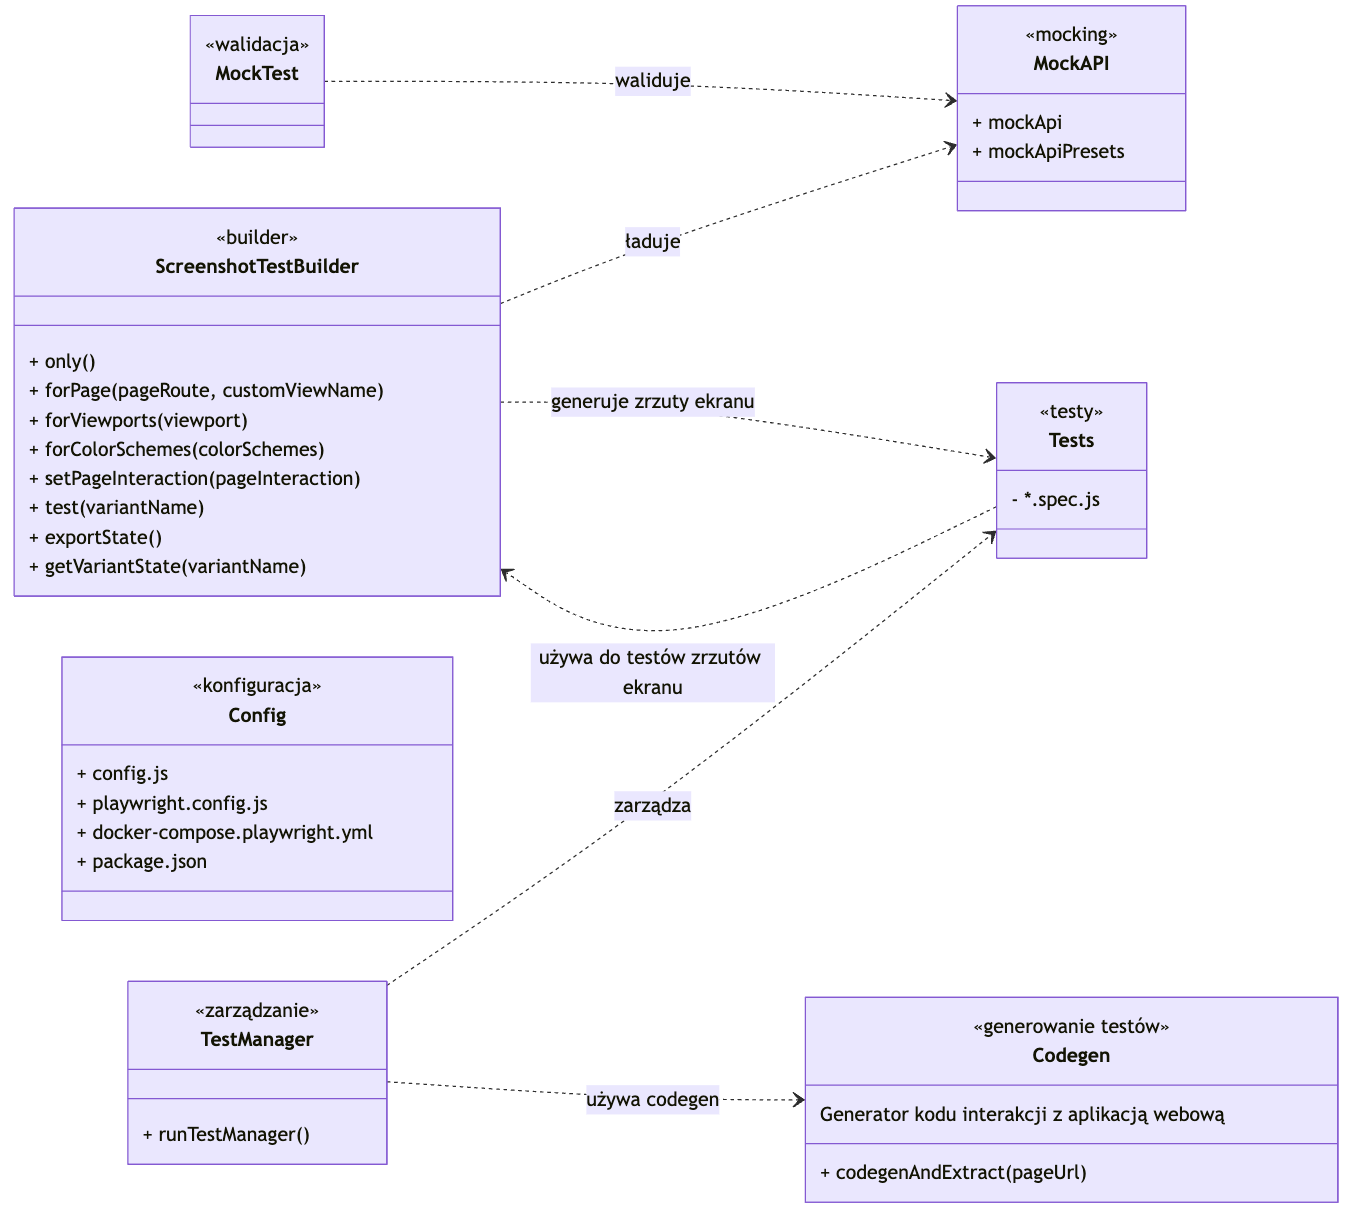
\includegraphics[width=0.95\textwidth]{diagram-projekt.png}
    \caption{Diagram klas wygenerowany w Mermaid}
    \label{fig:diagram-projekt}
\end{figure}

Na powyższym diagramie zaprezentowano również interakcje klas, takie jak:
\begin{itemize}
    \item \texttt{ScreenshotTestBuilder} współpracuje z \texttt{MockAPI} w celu ładowania danych i tworzenia zrzutów ekranu.
    \item \texttt{TestManager} używa \texttt{Codegen} do generowania kodu testów.
    \item \texttt{MockTest} służy do walidacji spójności między danymi testowymi a zasobami API.
\end{itemize}

\subsection{Diagram przypadków użycia}
\label{subsec:diagram-use}
Kolejnym istotnym elementem projektu jest \textbf{diagram przypadków użycia} (\autoref{fig:use-uml}), wskazujący na ogólny przepływ interakcji pomiędzy użytkownikiem (np. programistą lub testerem) a systemem. Przykładowo, „System CI/CD” może automatycznie uruchamiać testy przy każdym \emph{pushu} do repozytorium i wykorzystywać w tym celu gotowe skrypty wygenerowane przez nasze narzędzie.

\begin{figure}[H]
    \centering
    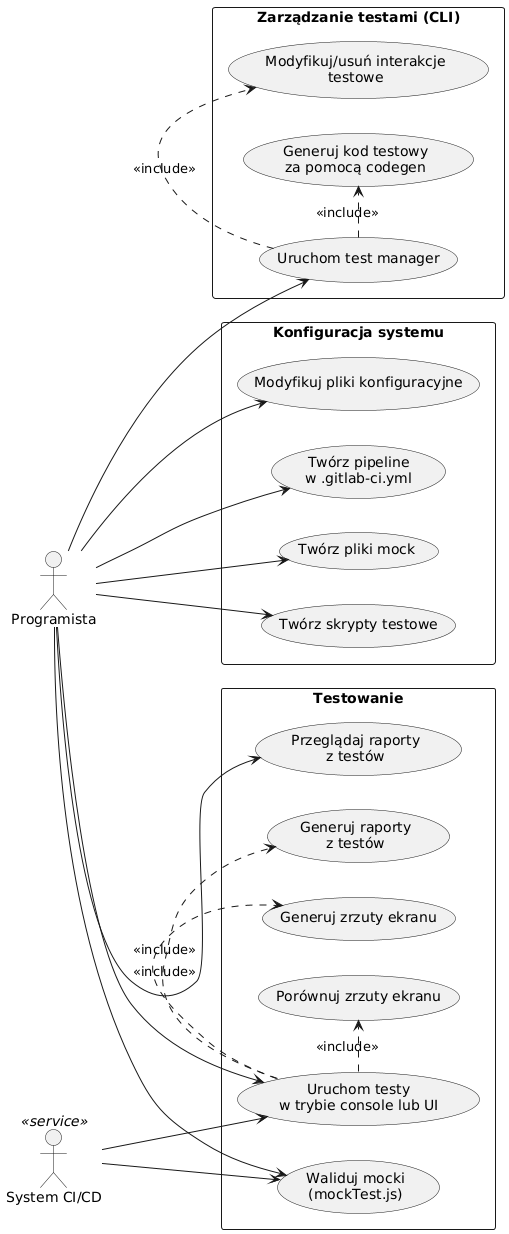
\includegraphics[width=0.9\textwidth]{use-uml.png}
    \caption{Diagram przypadków użycia wygenerowany w PlantUML}
    \label{fig:use-uml}
\end{figure}

Diagram prezentuje także rozszerzone akcje w \texttt{TestManager}, takie jak:
\begin{itemize}
    \item \emph{Generowanie kodu} (Codegen) w oparciu o zarejestrowane kroki,
    \item \emph{Modyfikacje i usuwanie interakcji}, np. gdy któryś z kroków staje się nieaktualny.
\end{itemize}

W następnych rozdziałach opisano w szczegółach implementację poszczególnych modułów (zarówno w zakresie kodu źródłowego, jak i logiki generującej
scenariusze testowe), a także zaprezentowano sposoby integracji z zewnętrznymi narzędziami, np. GitLab CI czy Jenkinsem.

\section{Interfejs użytkownika}
{Zaprezentuj, jak wygląda interfejs (graficzny lub konsolowy) Twojej aplikacji:
\begin{itemize}
    \item główne ekrany/formularze,
    \item sposób nawigacji,
    \item kluczowe funkcje (np. generowanie pliku testowego, zapis ustawień).
\end{itemize}
Możesz dołączyć zrzuty ekranu i omówić je.}

\chapter{Omówienie kodu źródłowego aplikacji}
{Przedstaw strukturę plików oraz folderów oraz wyjaśnij najważniejsze fragmenty implementacji. Wskaż, które biblioteki z rozdziału o „Dostępnych technologiach” zostały wykorzystane i w jaki sposób.}

\section{Struktura projektu}
{Opisz, w jaki sposób podzieliłeś/łaś projekt na moduły, pakiety, foldery:
\begin{itemize}
    \item logika generowania testów,
    \item definicja modelu danych (np. dane o testach, konfiguracje),
    \item klasy pomagające w tworzeniu raportów lub integracji z CI.
\end{itemize}}

\section{Kluczowe fragmenty kodu}
{Zademonstruj przykłady najważniejszych funkcji/metod, np.:
\begin{itemize}
    \item kod odpowiedzialny za rejestrowanie interakcji,
    \item generowanie plików testowych,
    \item konwersję danych do konkretnych frameworków.
\end{itemize}
Przedstaw je w formie listingów z krótkim komentarzem.}

\chapter{Przykłady użyć aplikacji}
{W tym rozdziale możesz zaprezentować, jak Twoje narzędzie działa w praktyce.}

\section{Uruchamianie narzędzia w trybie interaktywnym}
{Pokaż krok po kroku, jak użytkownik wypełnia formularz czy wybiera opcje w CLI, aby wygenerować testy. Zademonstruj końcowe pliki testowe.}

\section{Integracja z procesem CI/CD}
{Wyjaśnij, jak można włączyć wygenerowane testy do automatycznego pipeline’u, np. w GitLab CI, Jenkinsie, itp. Przedstaw przykładowy fragment konfiguracji.}

\chapter{Podsumowanie}
{Na koniec podsumuj swoją pracę, oceń jej efekty i zaproponuj kierunki rozwoju.}

\section{Wnioski końcowe}
{Opisz, w jakim stopniu udało się osiągnąć założone cele, co było największym wyzwaniem, co dało najwięcej satysfakcji/rezultatów.}

\section{Możliwości dalszego rozwoju}
{Opisz, jakie jeszcze funkcjonalności można by dodać do narzędzia, jakie usprawnienia byłyby przydatne, jakie biblioteki lub technologie mogłyby zostać wykorzystane w przyszłości.}

\begin{thebibliography}{9}
    \bibitem{roman2024} Roman, A., \& Zmitrow, K. (2024). \textit{Testowanie oprogramowania w praktyce: studium przypadków 2.0}.
    \bibitem{osherove2024} Osherove, R. (2024). \textit{Testy jednostkowe: świat niezawodnych aplikacji}.
    \bibitem{roman2024_case} Roman, A., \& Zmitrow, K. (2024). \textit{Testowanie oprogramowania w praktyce: studium przypadków}.
    \bibitem{roman2024_quality} Roman, A. (2024). \textit{Testowanie i jakość oprogramowania: modele, techniki, narzędzia}.
    \bibitem{circleci} CircleCI. (n.d.). What is End-to-End Testing? Pozyskano z \url{https://circleci.com/blog/what-is-end-to-end-testing/}
    \bibitem{playwright} Microsoft Playwright. (n.d.). Introduction to Playwright. Pozyskano z \url{https://playwright.dev/docs/intro}
\end{thebibliography}

\end{document}
